\begin{section}{Implementation and Power Spectra}
  \label{sec:simulation}
  We use \textsc{CUBEP$^3$M} \citep{bib:Harnois2013} to run
  140 simulations with a box size of 600 Mpc/$h$ and $512^3$ particles.
  For these simulations, we use cosmological
  parameters $\Omega_m=0.321$, $\Omega_{\Lambda}=1-\Omega_m=0.679$,
  $h=0.67$, $\sigma_8=0.83$, and $n_s=0.96$.
  The initial conditions are computed by
  transfer function \citep{bib:Lewis2000}
  at $z=100$.
  Zel'dovich
  approximation is used to calculate the displacement and initial velocities
  of particles.

  \begin{figure*}
    \centering
    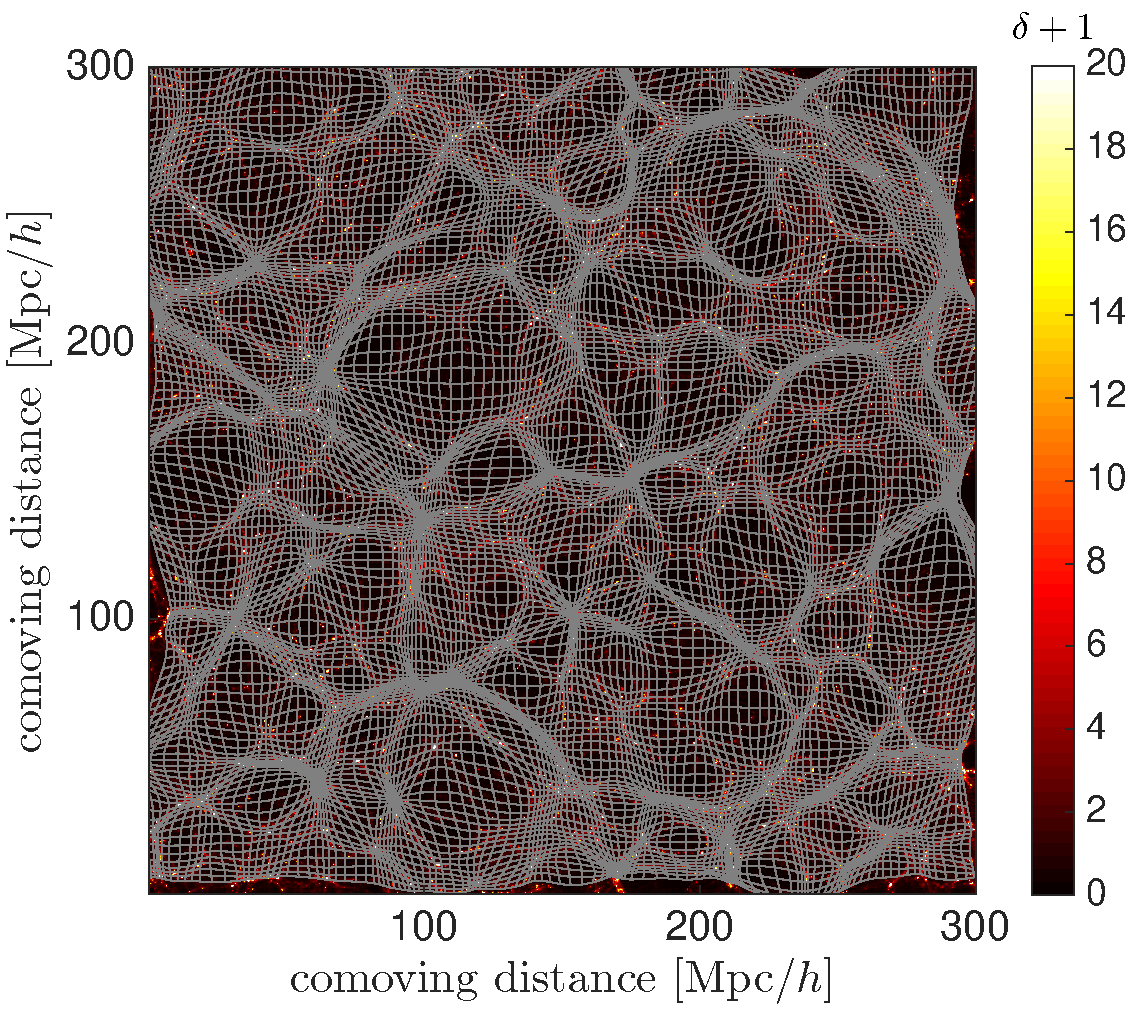
\includegraphics[width=0.9\textwidth]{fig1.pdf}
    \caption{ Illustration of IMC reconstruction.
      The 2-D projection of one layer of the deformed mesh of a sample
      $N$-body simulation is shown as curved white lines.  The
      density $\rho/\langle\rho\rangle=1+\delta$ on the mesh is shown
      underneath. For clarity, the scale of the density field is cut to 
      300 Mpc/$h$, and only every other grid line is plotted.}
    \label{fig:simandrec}
 \end{figure*}

 We use the Voronoi tessellation method \citep{bib:Van1994} to estimate the density contrast
 $\delta_N=\rho/\langle\rho\rangle-1$ ($N$ stands for nonlinear) from particle distributions, and apply the
 IMC reconstruction to these fields with $512^3$ grids.
 The reconstruction code solves the displacement potentials iteratively
 until the root mean square (rms) of the results drop from $\sim 7.5$
 to 0.20. The compression limiter is set to be 0.1 \citep{bib:Pen1995, bib:Pen1998,bib:ZhuH2016}. 
 For different simulation samples, a different number of
 iterations are required to get the results of the same rms. A total of
 130 simulations converged to the target rms within 2000 iterations, 
 and we use these results for the calculation in this paper.
 A 2-D projection
 of one layer of the deformed mesh and the original density field on
 the mesh are shown in Fig.~\ref{fig:simandrec}. 
 As expected, the deformed mesh traces the structure very well and
 the deformed grids do not cross each other, even in the 2-D projection.
 
 We study the Fisher information in the matter power
 spectra. More generally,
 the cross power spectrum $P_{\alpha\beta}(k)$ for species $\alpha$ and $\beta$
 ($\alpha=\beta$ for auto power spectrum) is defined as
 \begin{align}
   \langle \delta_\alpha^\dagger(\bm{k})\delta_\beta(\bm{k}') \rangle =
   (2\pi)^3 P_{\alpha\beta}(k) \delta_{\rm {3D}}(\bm{k}-\bm{k}'),
 \end{align}
 where $\delta_{\alpha}$ and $\delta_{\beta}$ are any two fields and
 $\delta_{\rm{3D}}$ is the three-dimensional Dirac delta function. We typically consider instead
 the dimensionless power spectrum, $\Delta_{\alpha\beta}^2(k)$, defined as
 \begin{align}
   \Delta_{\alpha\beta}^2(k) \equiv \frac{k^3 P_{\alpha\beta}(k)}{2\pi ^2}.
 \end{align}
 In the left panel of Fig.~\ref{fig:cp}, we show the matter auto power
 spectrum of linear theory density fields $\delta_L$, nonlinear density
 fields ($\delta_N$) from simulations and reconstructed density fields
 (from Eq. \ref{eq:delta}).  For the simulation
 results, we use the average value of all 130 simulations and show
 $1\sigma$ standard deviations as error bars.  

 To quantify the cross-correlation
 between fields, we compute the cross correlation coefficient
 $r_{\alpha\beta}(k)\equiv P_{\alpha\beta}/\sqrt{P_{\alpha\alpha}P_{\beta\beta}}$.  In the right panel of
 Fig.~\ref{fig:cp}, we show $r_{NL}$ and $r_{RL}$.  We see that, compared with $\delta_N$,
 $\delta_R$ correlates with $\delta_L$ on much wider range of scales.
 We compare our reconstruction correlation coefficient to that of the $E$-mode 
 reconstruction, $r_{EL}$, 
 %,($\delta_E(\bs{q})= - \nabla_q \cdot \bs{\Psi}(\bs{q})$) 
 computed in \citealt{bib:Yu2016}.
 Even though $r_{RL}$ decreases from $r_{EL}$ in the nonlinear regime due to the fact that the IMC reconstruction 
 cannot recover the shell-crossing present on these scales, we find that linear
 modes are recovered successfully on scales $k\simeq 0.05 - 0.3$ $h$/Mpc.
 Specifically, the scale where $r(k)=1/2$ increases from $k\simeq 0.2$ $h$/Mpc to
 $0.8$ $h$/Mpc after reconstruction.  In comparison with the results of \citet{bib:ZhuH2016},
 which showed $r(k\simeq0.9 h/\rm{Mpc})=1/2$, we find the correlation coefficient falls off at slightly lower
 wave numbers, which we attribute to using fewer particles per simulation.

  \begin{figure*}
    \centering
    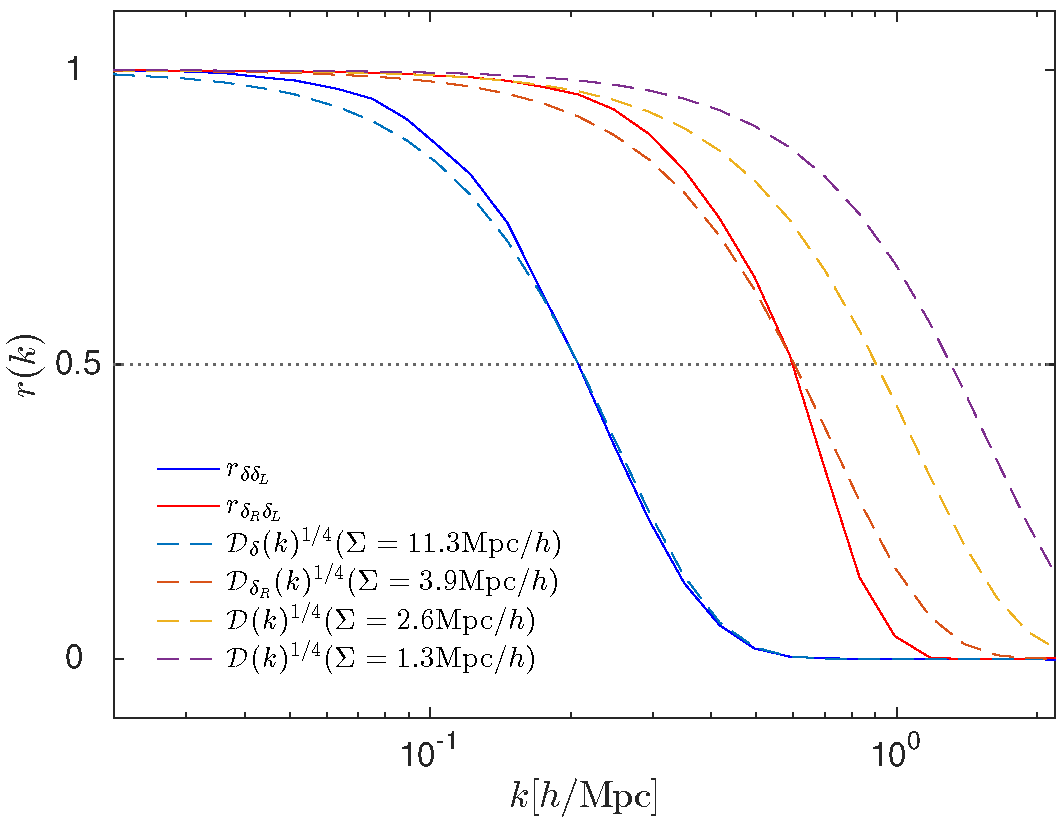
\includegraphics[width=0.5\textwidth]{fig2a.pdf}
    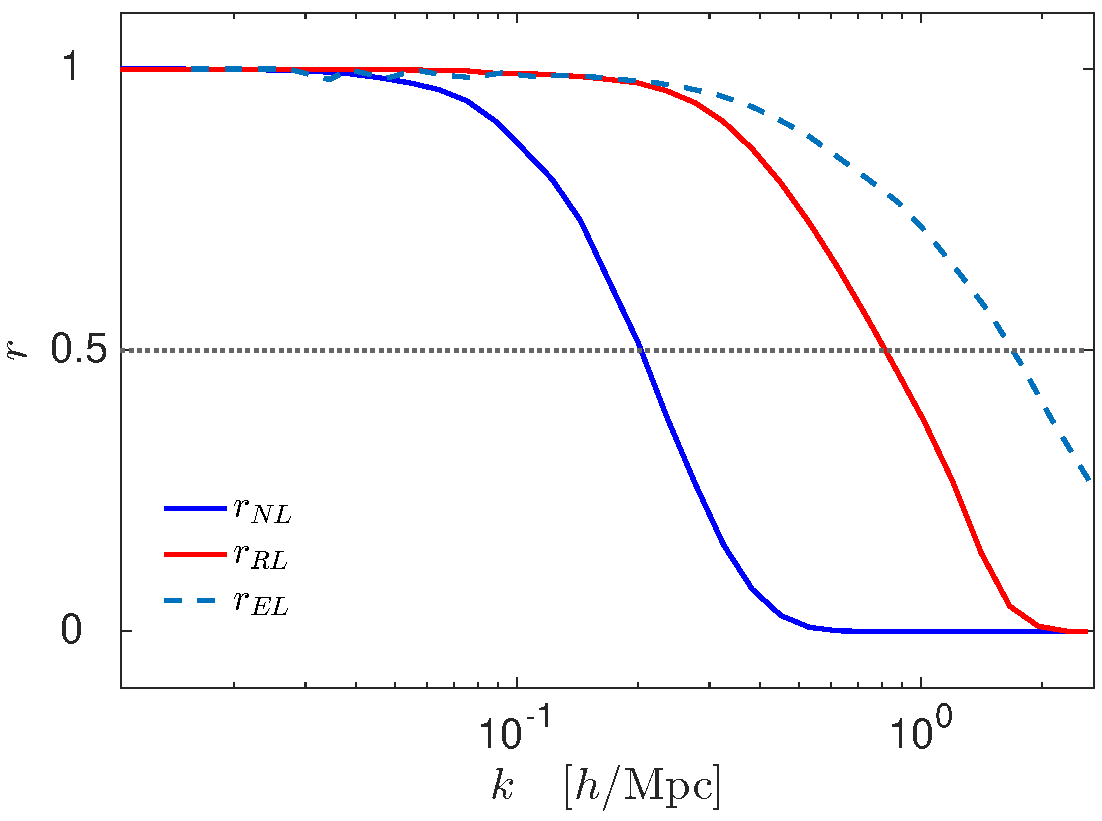
\includegraphics[width=0.485\textwidth]{fig2b.pdf}
    \caption{{\it Left.} The dimensionless power spectrum computed via
      linear theory (black dash-dotted line), the mean value of 130 $N$-body
      simulations with $1\sigma$ error bars (blue solid line), and reconstruction
      of the simulations (red dashed line).  {\it Right.} The cross correlation
      coefficient between simulation and linear densities $r_{NL}$ (blue solid line),
      IMC reconstructed and linear densities $r_{RL}$ (red dashed line), and E-mode reconstruction $r_{EL}$ (cyan dotted line) from \citealt{bib:Yu2016}.}
    \label{fig:cp}
  \end{figure*}


\end{section}

